\newpage
\section{Results}
\subsection{Experimental Setup}
Executing the MapReduce workflow with different inputs, and configurations:
\begin{itemize}
  \item \textbf{Input size}: the size of the input file is varied to evaluate the performance of the MapReduce workflow.
        \begin{itemize}
          \item \textbf{Paradise Lost} $\sim$ 310 kB
          \item \textbf{Moby Dick} $\sim$ 421kB
          \item \textbf{Frankenstein} $\sim$ 440 kB
          \item \textbf{Divina Commedia} $\sim$ 600 kB
          \item \textbf{Gerusalemme Liberata} $\sim$ 691 kB
          \item \textbf{Promessi Sposi} $\sim$ 1.440 kB
          \item \textbf{Test file} (random generated sequence of char) of $\sim$ 800 MB.
        \end{itemize}
  \item \textbf{Number of mappers}: Hadoop handles this step
  \item \textbf{Number of reducers}: From one up to three reducers are used for letter frequency
\end{itemize}

\subsection{Performance Analysis}
  
\begin{figure}[H]
  \centering
  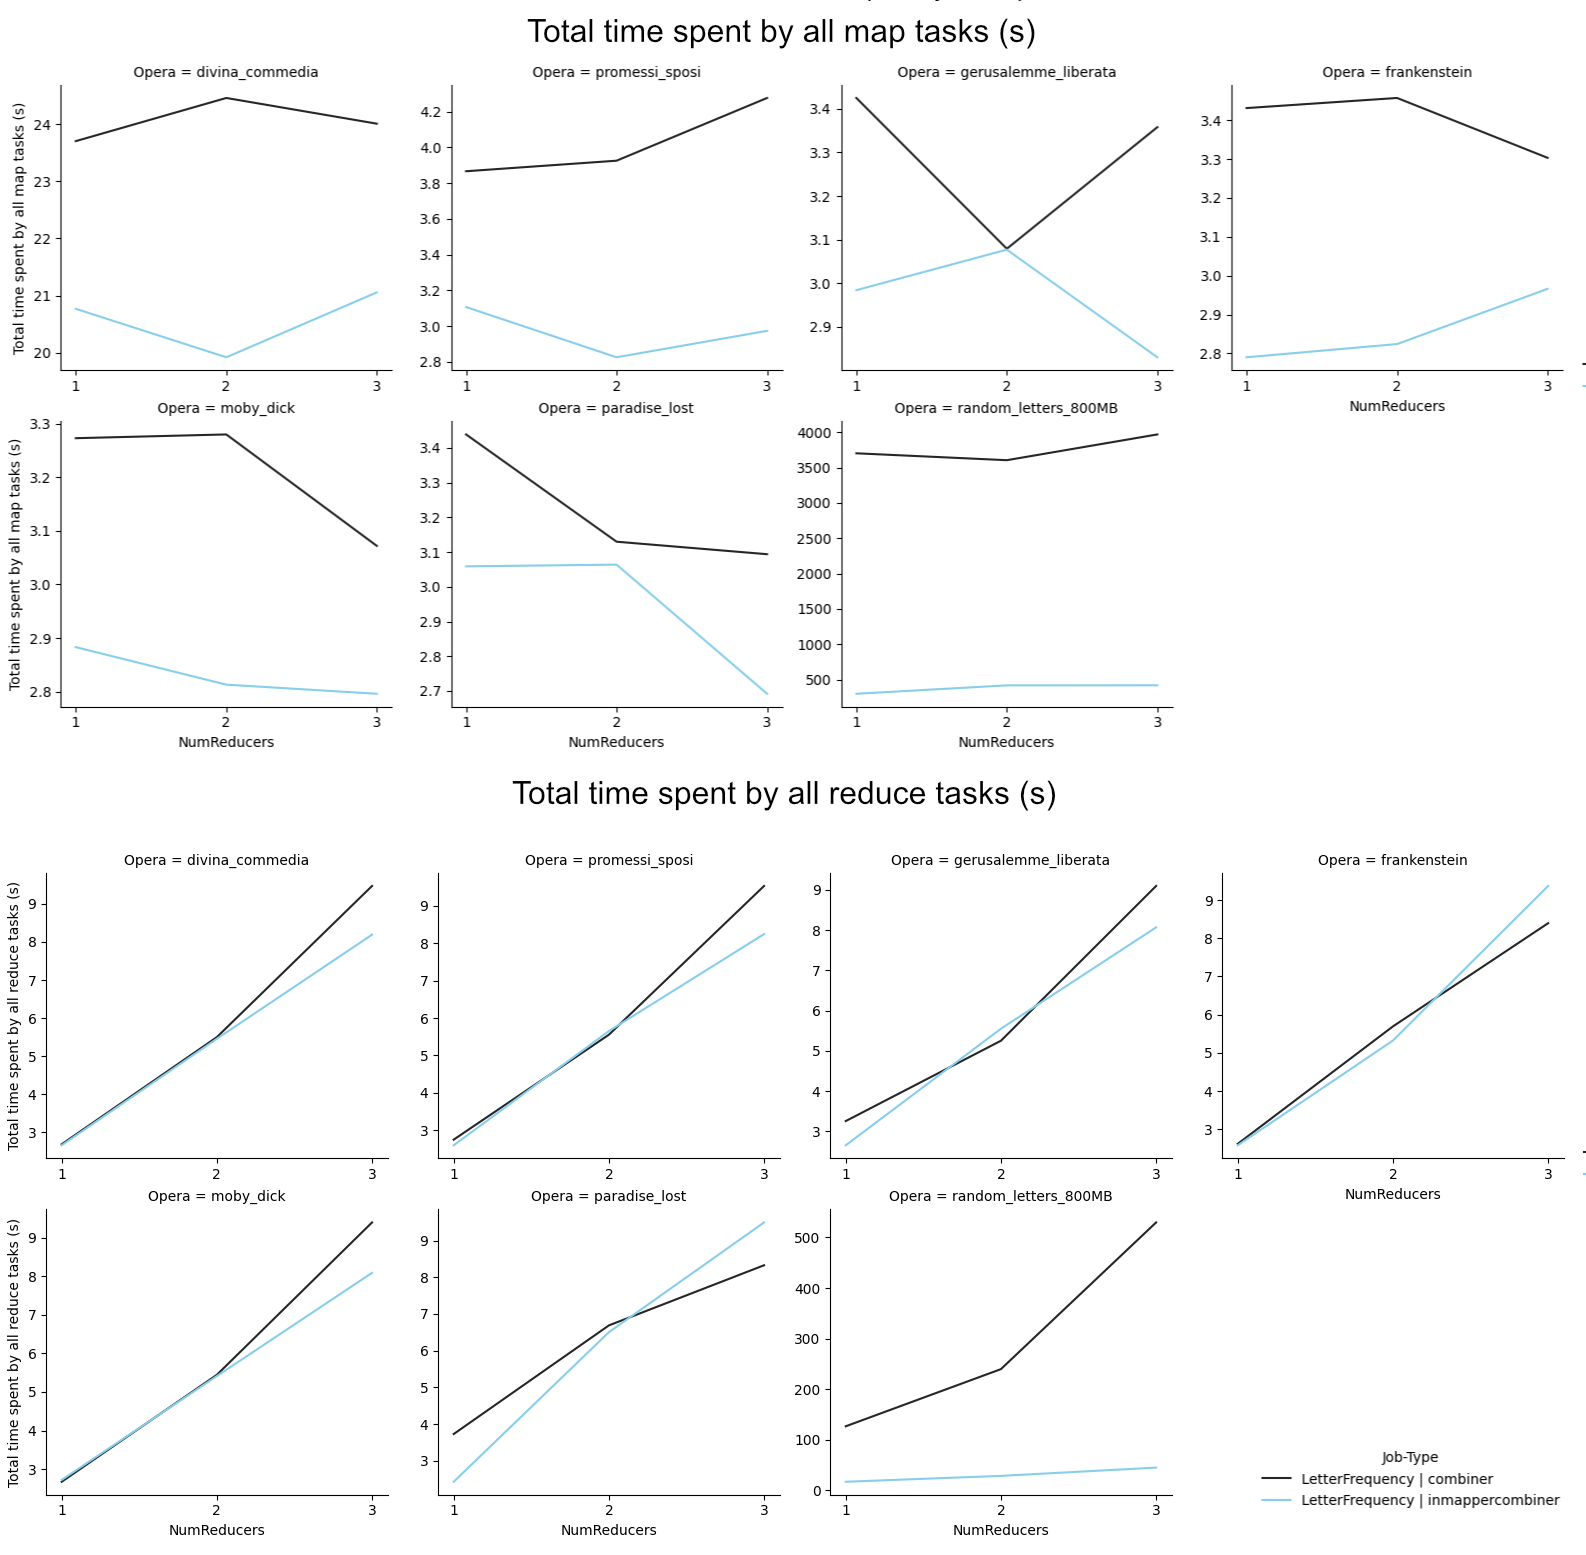
\includegraphics[width=0.8\textwidth]{media/performance/TotalTimeMapReduce.png}
  \caption{TotalTimeMapReduce}
  \label{fig:TotalTimeMapReduce}
\end{figure}

\begin{figure}[H]
  \centering
  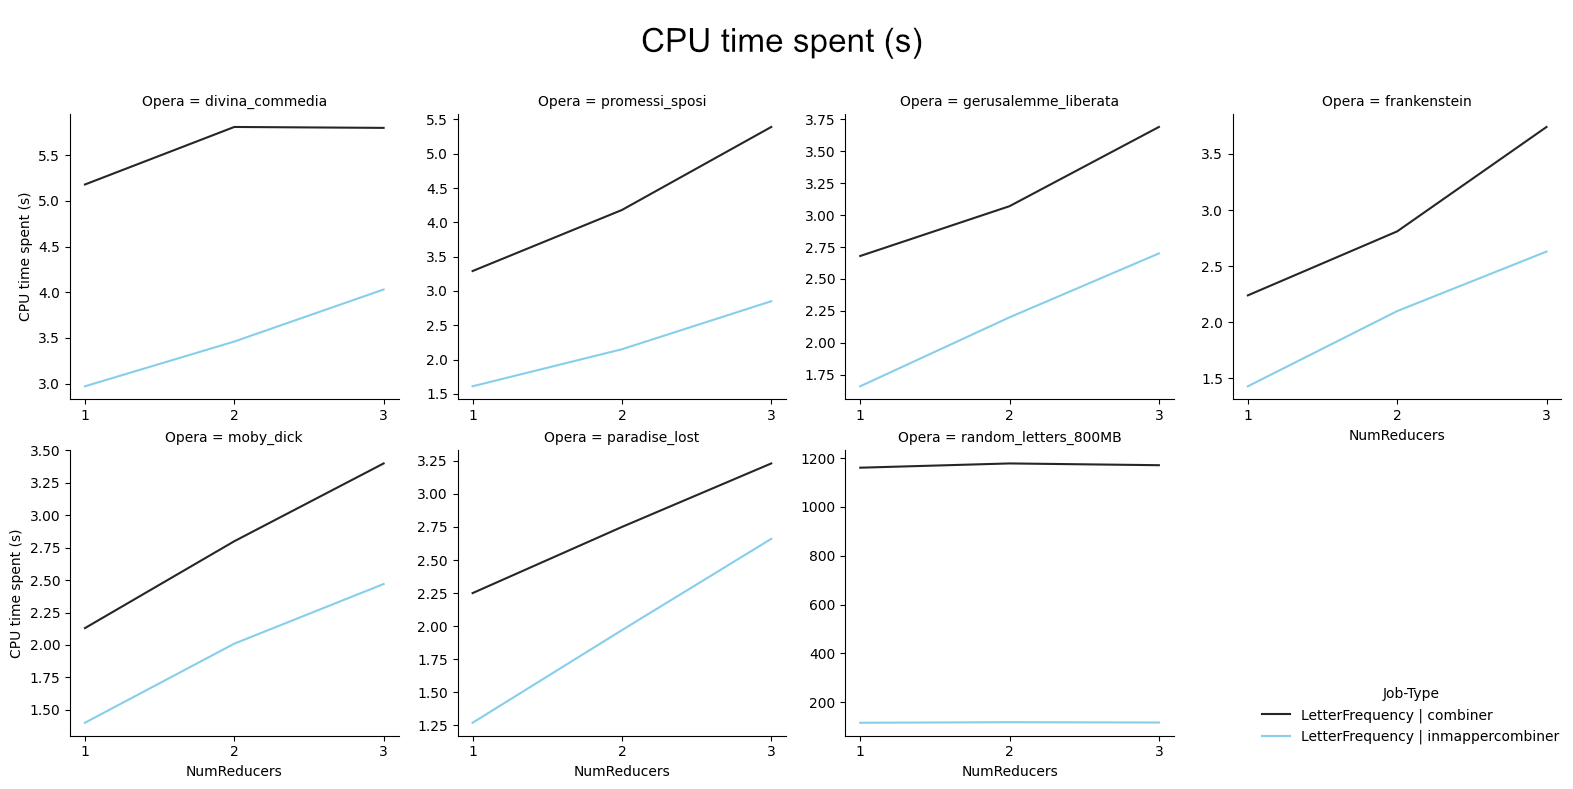
\includegraphics[width=0.8\textwidth]{media/performance/CpuTIME.png}
  \caption{Cpu Time}
  \label{fig:CpuTIME}
\end{figure}

\begin{figure}[H]
  \centering
  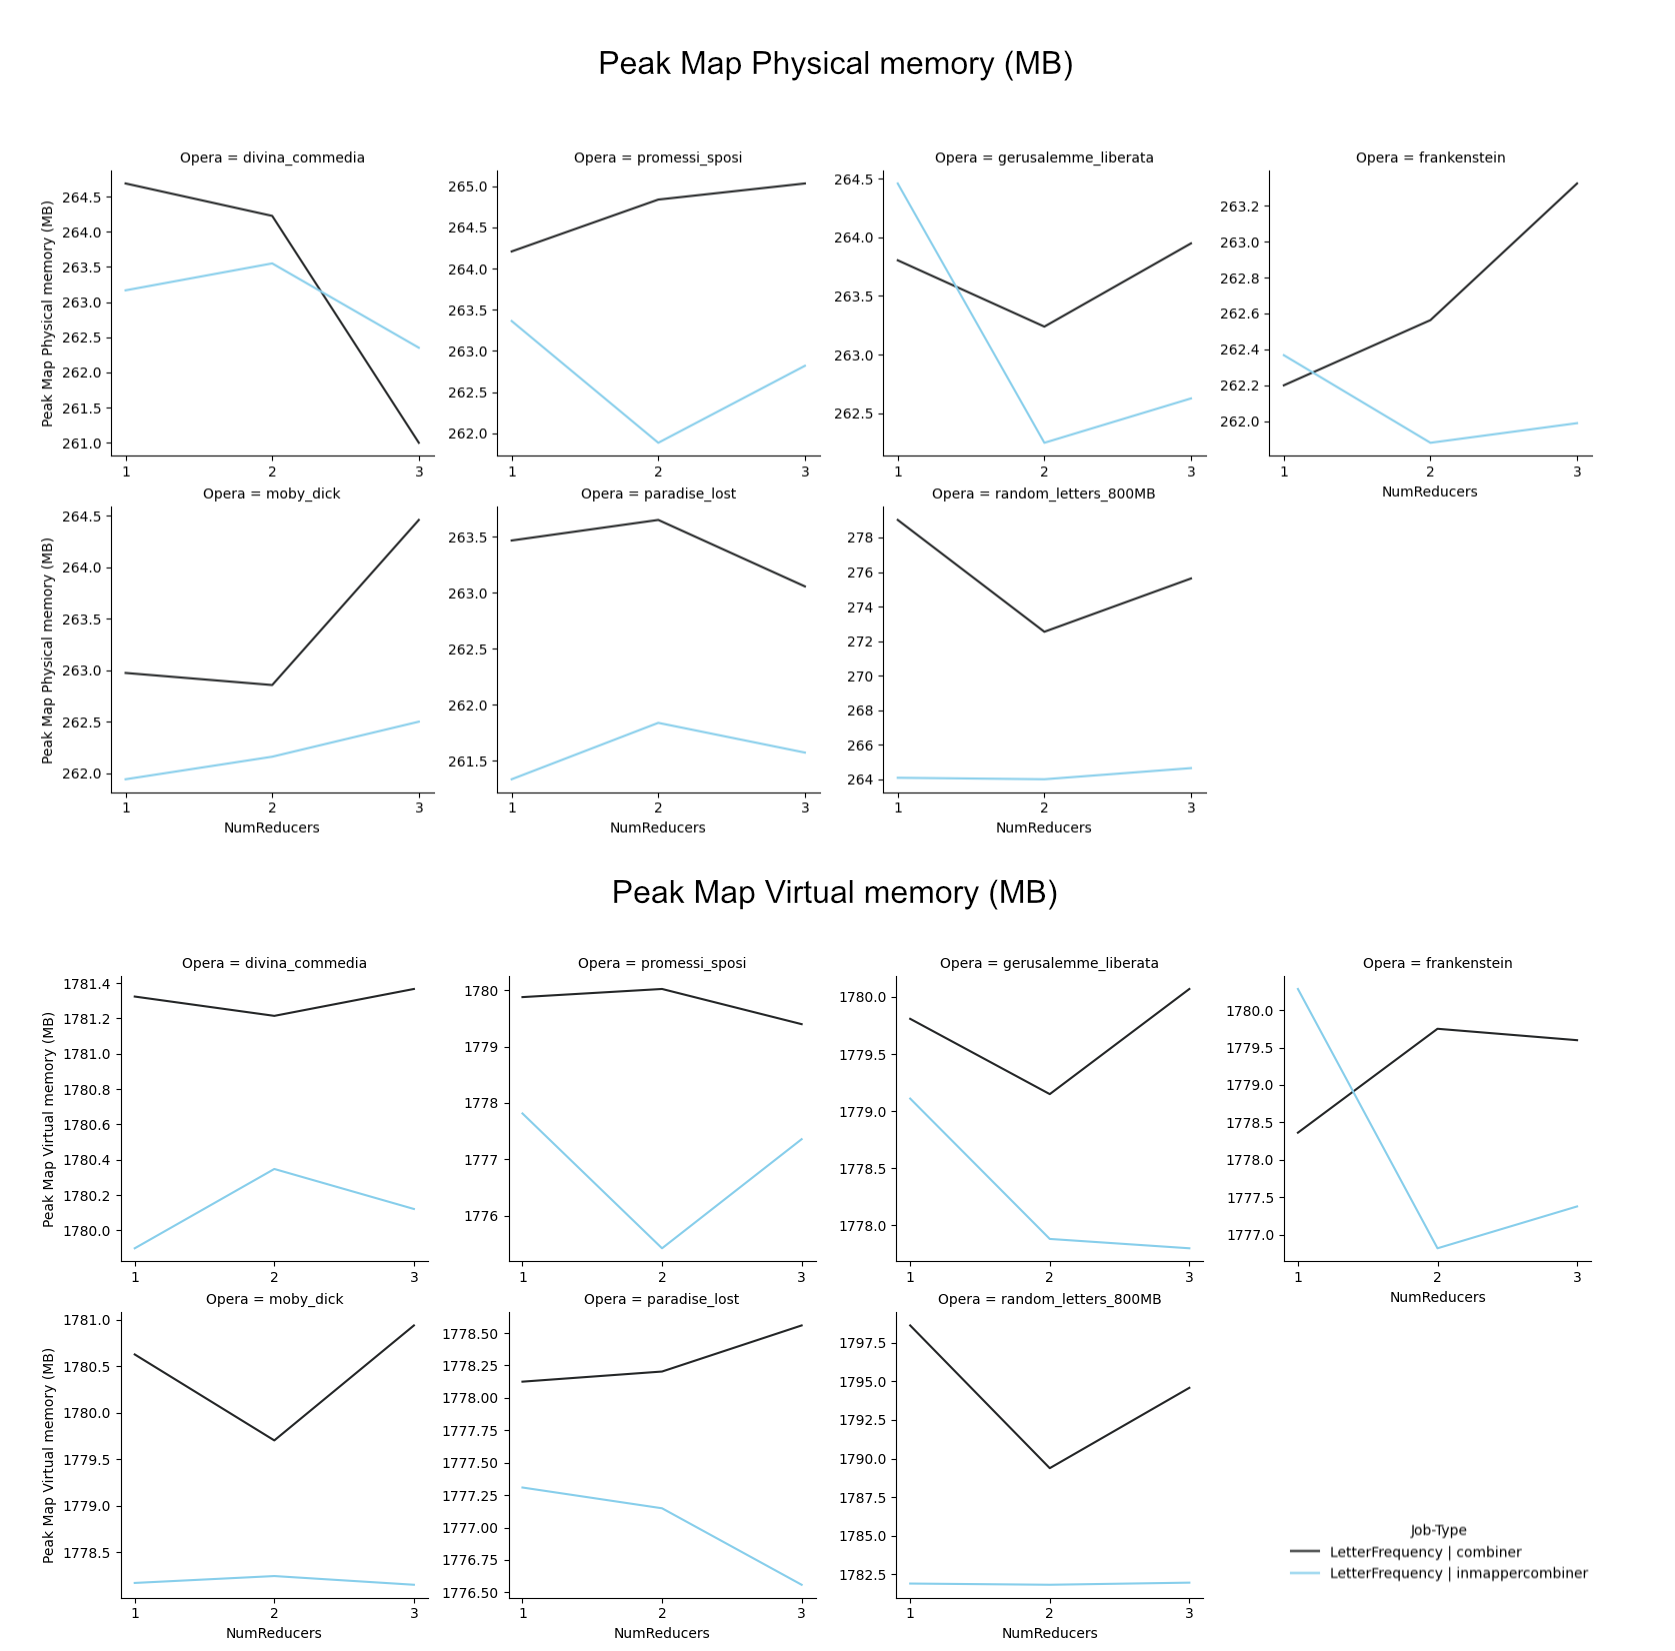
\includegraphics[width=0.8\textwidth]{media/performance/PeakMapMemory.png}
  \caption{Peak Map Memory}
  \label{fig:PeakMapMemory}
\end{figure}

\begin{figure}[H]
  \centering
  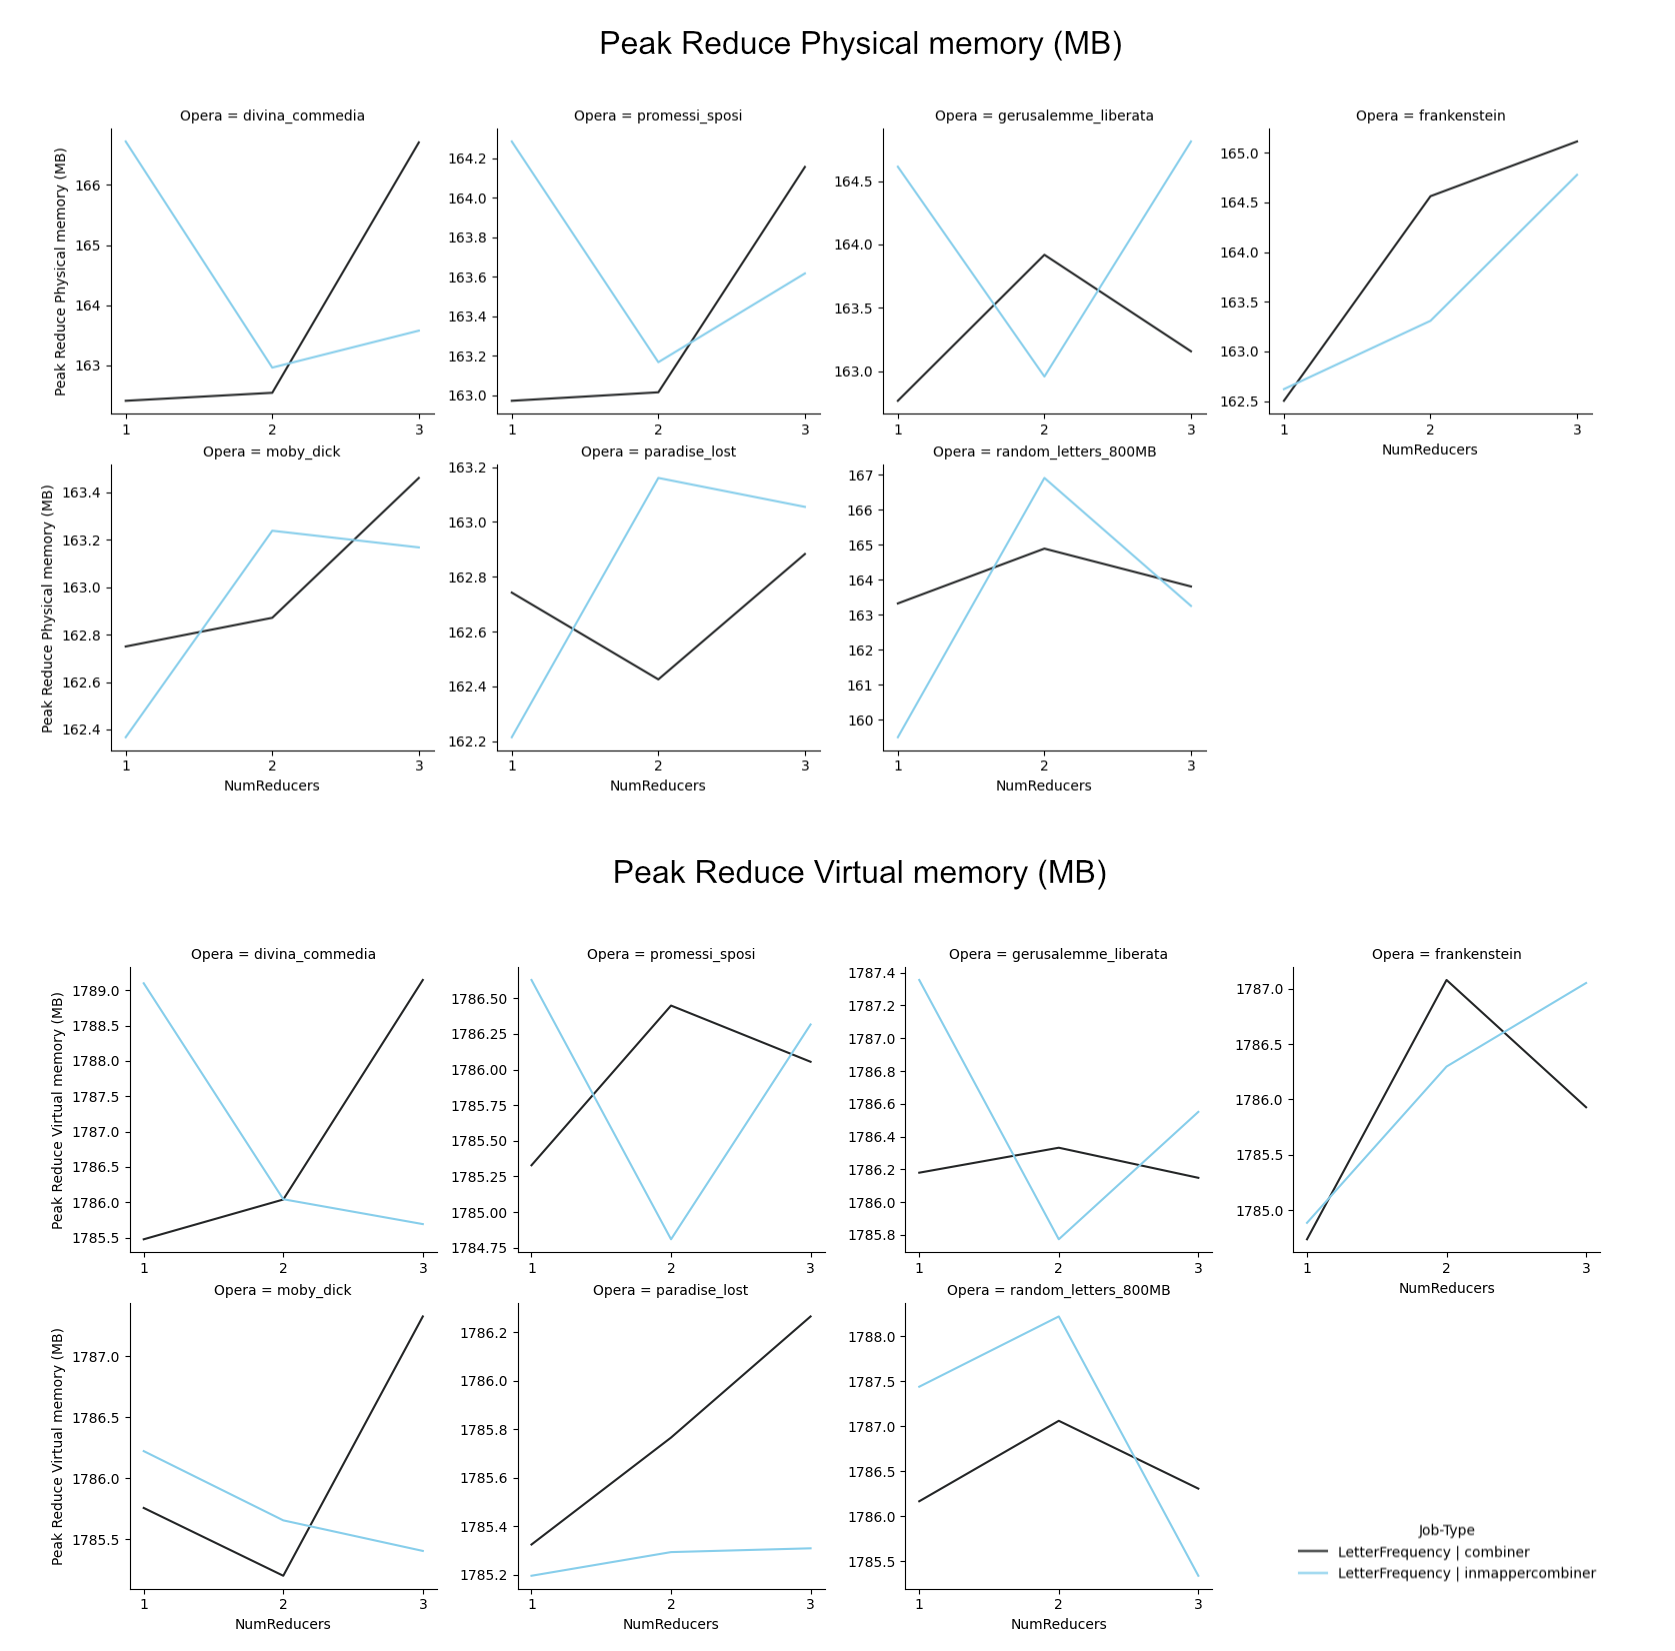
\includegraphics[width=0.8\textwidth]{media/performance/PeakReduceMemory.png}
  \caption{Peak Reduce Memory}
  \label{fig:PeakReduceMemory}
\end{figure}

\begin{figure}[H]
  \centering
  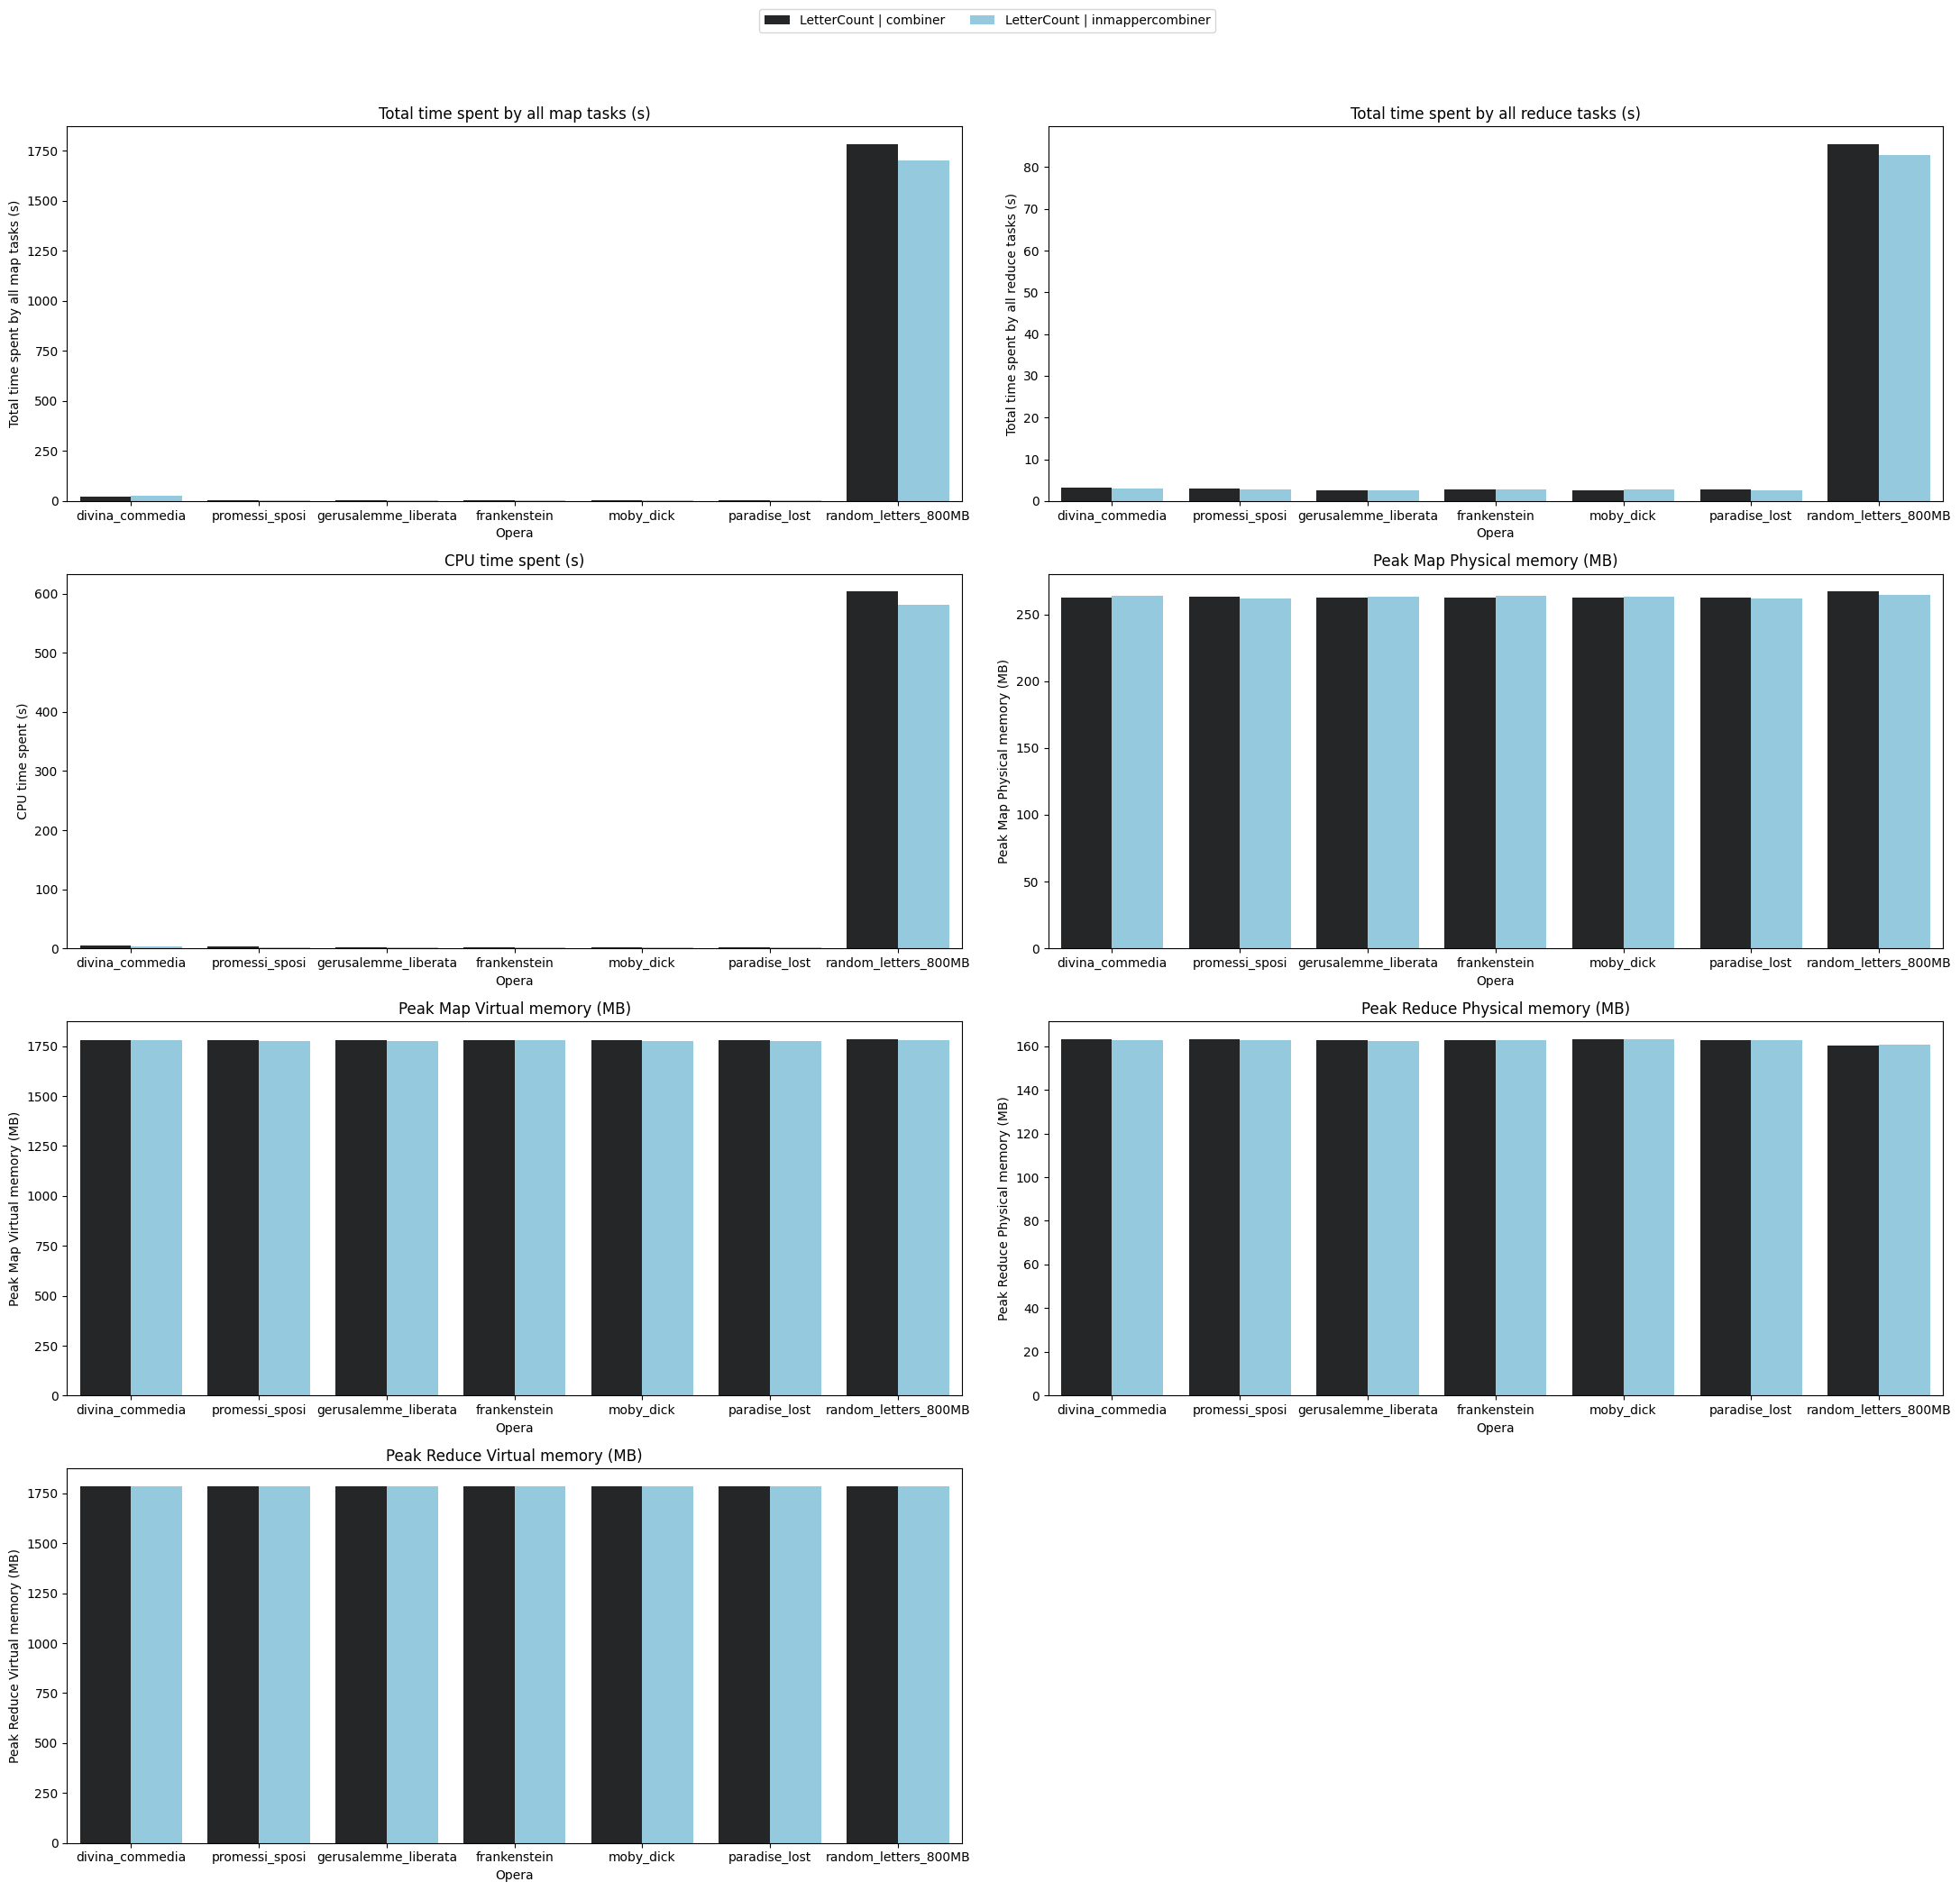
\includegraphics[width=0.8\textwidth]{media/performance/performance_LetterCount.png}
  \caption{Performance Letter Count}
\end{figure}

\newpage

\subsection{Letter Frequency Analysis}

\begin{figure}[H]
  \centering
  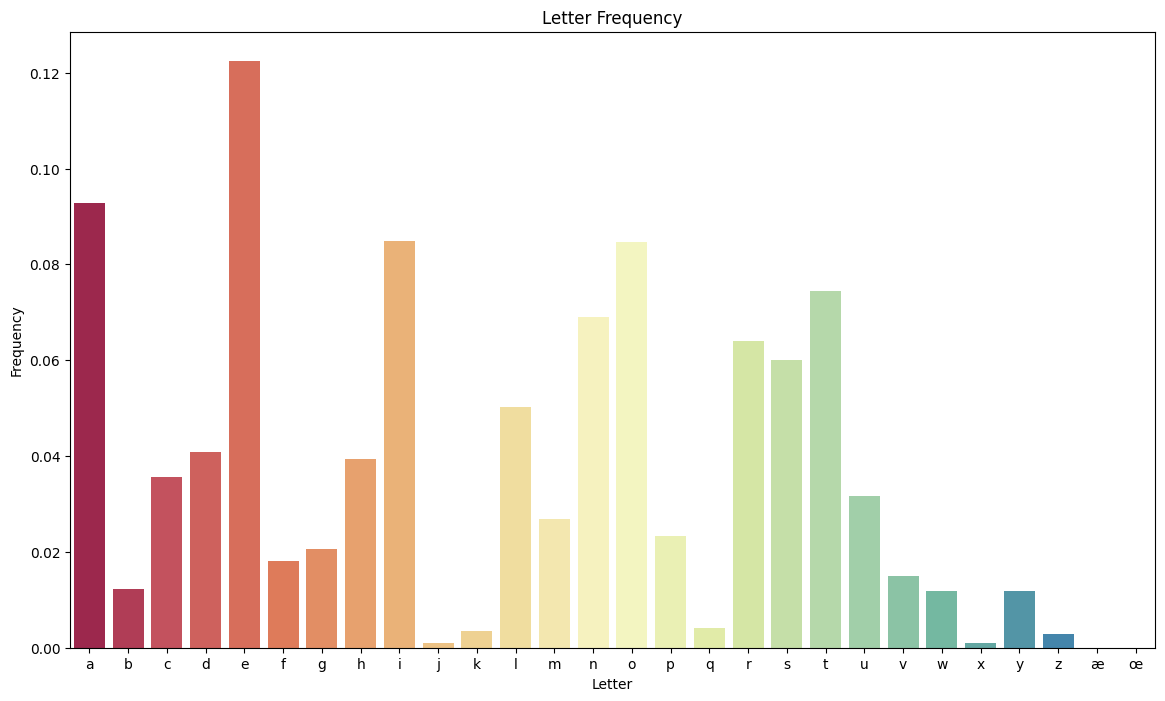
\includegraphics[width=0.8\textwidth]{media/qualitative analysis/letter_freq_dist.png}
  \caption{Letter Frequency Distribution}
  \label{fig:letter_freq_dist}
\end{figure}

\begin{figure}[H]
  \centering
  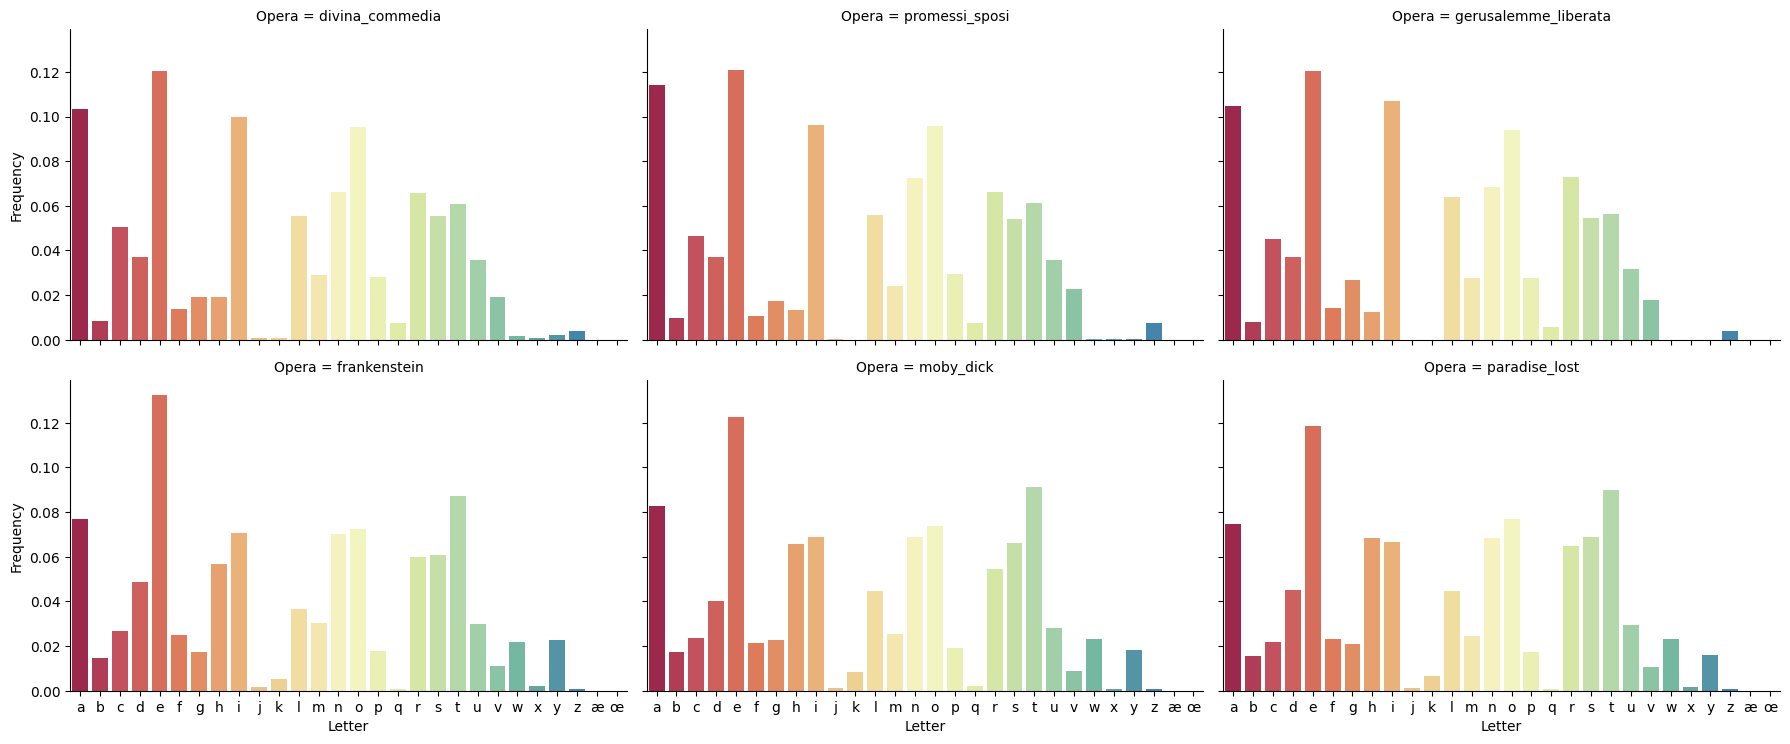
\includegraphics[width=0.9\textwidth]{media/qualitative analysis/letter_freq_dist_opera.png}
  \caption{Letter Frequency Distribution for different Operas}
  \label{fig:letter_freq_dist_opera}
\end{figure}

\begin{figure}[H]
  \centering
  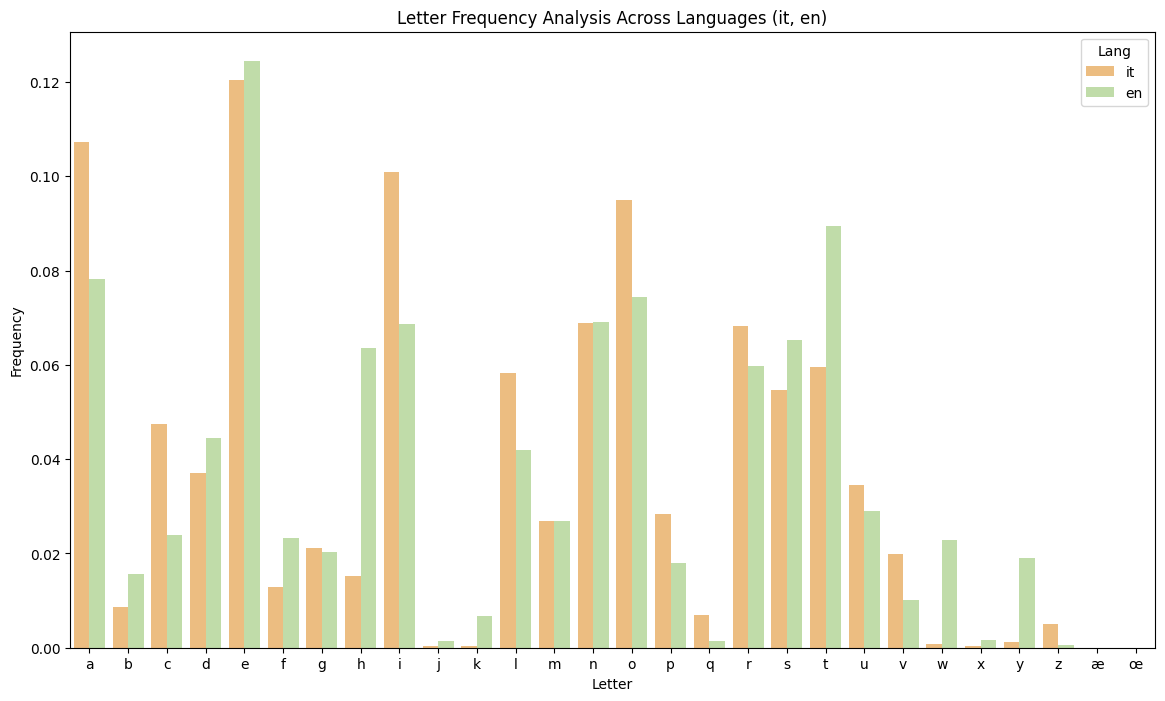
\includegraphics[width=0.8\textwidth]{media/qualitative analysis/letter_freq_dist_lang.png}
  \caption{Letter Frequency Distribution for italian and english}
  \label{fig:letter_freq_dist_lang}
\end{figure}

\begin{figure}[H]
  \centering
  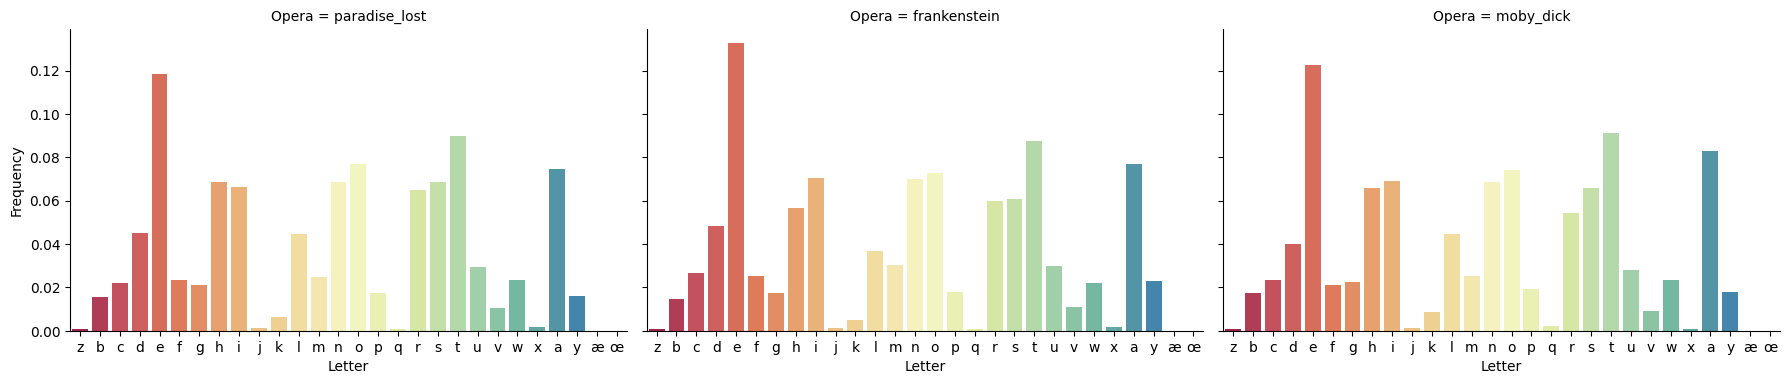
\includegraphics[width=0.9\textwidth]{media/qualitative analysis/letter_freq_dist_lang_en.png}
  \caption{Letter Frequency Distribution for english}
  \label{fig:letter_freq_dist_lang_en}
\end{figure}

\begin{figure}[H]
  \centering
  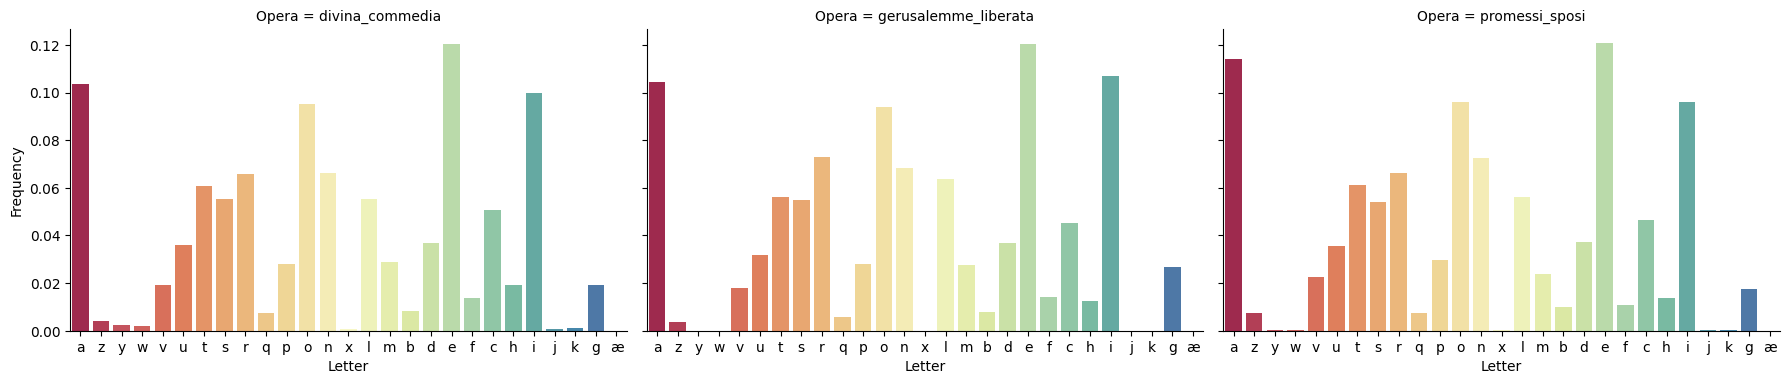
\includegraphics[width=0.9\textwidth]{media/qualitative analysis/letter_freq_dist_lang_it.png}
  \caption{Letter Frequency Distribution for italian}
  \label{fig:letter_freq_dist_lang_it}
\end{figure}

\begin{figure}[H]
  \centering
  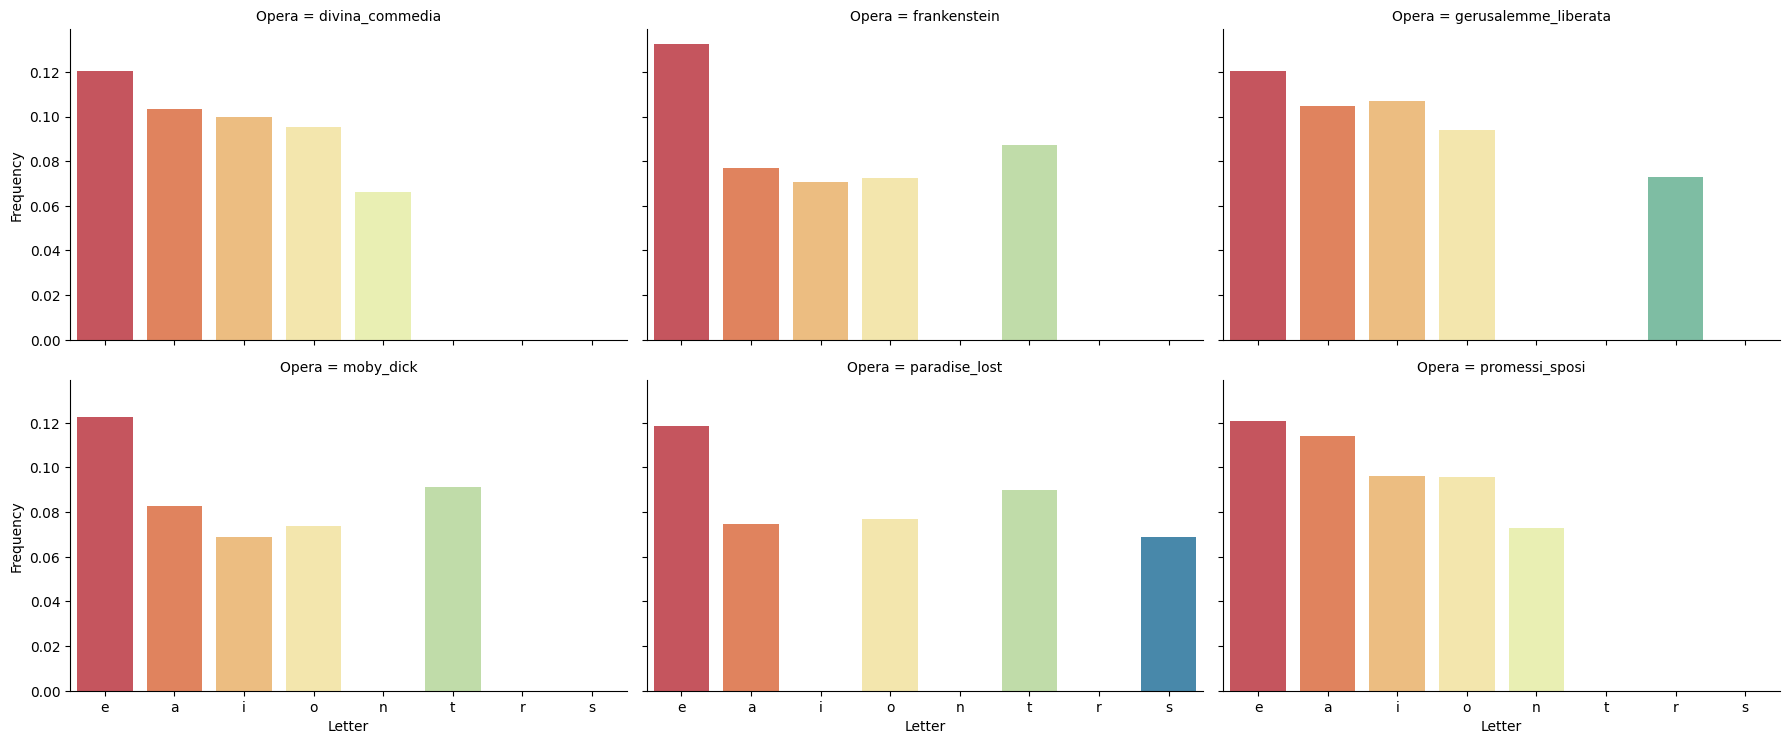
\includegraphics[width=1\textwidth]{media/qualitative analysis/top_5_letters.png}
  \caption{Top 5 letters}
  \label{fig:top_5_letters}
\end{figure}

